%%*************************************************************************
%% Legal Notice:
%% This code is offered as-is without any warranty either expressed or
%% implied; without even the implied warranty of MERCHANTABILITY or
%% FITNESS FOR A PARTICULAR PURPOSE! 
%% User assumes all risk.
%% In no event shall IEEE or any contributor to this code be liable for
%% any damages or losses, including, but not limited to, incidental,
%% consequential, or any other damages, resulting from the use or misuse
%% of any information contained here.
%%
%% All comments are the opinions of their respective authors and are not
%% necessarily endorsed by the IEEE.
%%
%% This work is distributed under the LaTeX Project Public License (LPPL)
%% ( http://www.latex-project.org/ ) version 1.3, and may be freely used,
%% distributed and modified. A copy of the LPPL, version 1.3, is included
%% in the base LaTeX documentation of all distributions of LaTeX released
%% 2003/12/01 or later.
%% Retain all contribution notices and credits.
%% ** Modified files should be clearly indicated as such, including  **
%% ** renaming them and changing author support contact information. **
%%
%% File list of work: IEEEtran.cls, IEEEtran_HOWTO.pdf, bare_adv.tex,
%%                    bare_conf.tex, bare_jrnl.tex, bare_jrnl_compsoc.tex
%%*************************************************************************

\documentclass[10pt,conference]{IEEEtran}


% Some very useful LaTeX packages include:
% (uncomment the ones you want to load)


% *** GRAPHICS RELATED PACKAGES ***
%
\ifCLASSINFOpdf
  \usepackage[pdftex]{graphicx}
  \usepackage{epstopdf}
  \PrependGraphicsExtensions{.eps}
  \graphicspath{{./figures/}}
  %\DeclareGraphicsExtensions{.eps}
  % \usepackage[pdftex]{graphicx}
  % declare the path(s) where your graphic files are
  % \graphicspath{{../pdf/}{../jpeg/}}
  % and their extensions so you won't have to specify these with
  % every instance of \includegraphics
  % \DeclareGraphicsExtensions{.pdf,.jpeg,.png}
\else
  % or other class option (dvipsone, dvipdf, if not using dvips). graphicx
  % will default to the driver specified in the system graphics.cfg if no
  % driver is specified.
  \usepackage[pdftex]{graphicx}
  \usepackage{epstopdf}
  % declare the path(s) where your graphic files are
  \graphicspath{{./figures/}}
  % and their extensions so you won't have to specify these with
  % every instance of \includegraphics
  \DeclareGraphicsExtensions{.eps}
\fi

% *** MATH PACKAGES ***
%
\usepackage[cmex10]{amsmath}

% *** PDF, URL AND HYPERLINK PACKAGES ***
%
\usepackage{url}

\hyphenation{op-tical net-works semi-conduc-tor}


\begin{document}

\title{A Revolutionary New Paradigm for the Reduction and Analysis of Astronomical Images}


\author{\IEEEauthorblockN{Scott Michael \IEEEauthorrefmark{1}, Patricia Knezek \IEEEauthorrefmark{2}, Elizabeth Stobie \IEEEauthorrefmark{3}, Robert Henschel \IEEEauthorrefmark{1} and Stephen Simms \IEEEauthorrefmark{1}}
\IEEEauthorblockA{\IEEEauthorrefmark{1}Indiana University\\
Bloomington, Indiana 47408\\
Email: scamicha@indiana.edu}
\IEEEauthorblockA{\IEEEauthorrefmark{2}WIYN Consortium Inc.\\
Tucson, Arizona 85726\\
Email: knezek@noao.edu}
\IEEEauthorblockA{\IEEEauthorrefmark{3}National Optical Astronomy Observatory\\
Tucson, Arizona 85726\\
Email: bstobie@noao.edu}}

% use for special paper notices
%\IEEEspecialpapernotice{(Invited Paper)}

% make the title area
\maketitle


\begin{abstract}
%\boldmath
In this article we propose a revolutionary new paradigm for the processing and analysis of astronomical image data. Included is a brief discussion of the current paradigm in astronomical image processing. We describe a blueprint for a centralized data repository and processing system, which leverages national cyberinfrastructure. The upcoming One Degree Imager (ODI) instrument, to be installed at the WIYN observatory in 2011, is examined as an ideal use case. Details on the major components and a detailed workflow in the case of data processing for the ODI instrument are included. 
\end{abstract}
% IEEEtran.cls defaults to using nonbold math in the Abstract.
% This preserves the distinction between vectors and scalars. However,
% if the conference you are submitting to favors bold math in the abstract,
% then you can use LaTeX's standard command \boldmath at the very start
% of the abstract to achieve this. Many IEEE journals/conferences frown on
% math in the abstract anyway.

% no keywords
\begin{IEEEkeywords}
Image processing, Image analysis, Astronomy, Pipeline processing
\end{IEEEkeywords}



% For peer review papers, you can put extra information on the cover
% page as needed:
% \ifCLASSOPTIONpeerreview
% \begin{center} \bfseries EDICS Category: 3-BBND \end{center}
% \fi
%
% For peerreview papers, this IEEEtran command inserts a page break and
% creates the second title. It will be ignored for other modes.
\IEEEpeerreviewmaketitle

\section{Introduction}\label{sec:intro}

One of the principle methods of scientific discovery in astronomy is via the analysis of astronomical images. Following the replacement of photographic plates by charged-coupled devices (CCDs) in the 1970s and 1980s, the role of specialized astronomical software in image reduction and analysis has grown steadily. Today, typical CCD imagers are 8K$\times$8K pixels in size or smaller, and the output data volume is fairly small by most standards. Because of this, the reduction and analysis processes are carried out by individual researchers using their own computational and storage resources. Many national entities (e.g. the National Optical Astronomy Observatory (NOAO) and NASA) have devoted resources to developing and supporting software packages for image analysis that can be run on personal resources.  

However, cutting-edge instruments that are just beginning to come online, as well as instruments planned for the not too distant future will produce data in volumes that a single investigator can not hope to store, analyze, and archive on their own. Currently, the Pan-STARRS gigapixel imager is producing more than 1 TB of data per day. The Solar Dynamics Observatory, a space based observatory, transmits 1.5 TB of raw data to the ground every day. Other instruments in their design or construction phases include the One Degree Imager, capable of producing 4 TB per day; the Large Synoptic Sky Survey, which will produce 30 TB of data per day; and the Joint Dark Energy Mission, a space based observatory capable of producing several terabytes of data per day. Clearly, these data volumes are much larger than the typical astronomer is accustomed to dealing with and most observational astronomers lack access to the resources that would be required to handle these amounts of data.

To address this changing landscape of data output from leading scientific observatories, we propose a new paradigm for the storage, analysis and archiving of astronomical digital image data. By taking advantage of national cyberinfrastructure and the parallel nature of image processing, the burden of storing, managing, and processing the data can be moved from the individual to more capable supercomputing resources.  

The rest of this paper is arranged as follows: section \ref{sec:current} describes the current paradigm employed by astronomers for dealing with imaging data and outline some upcoming problems with this paradigm. We detail a new paradigm for the processing of astronomical images in section \ref{sec:rev}. In section \ref{sec:ODI} we describe how this new paradigm applies to the ODI instrument. Finally, in section \ref{sec:future} we explore possible future directions and in section \ref{sec:conclusions} we present our final conclusions.

\section{The Current Paradigm for the Reduction of Astronomical Images}\label{sec:current}

Today most of the hundreds of astronomical optical imaging instruments at medium to large scale observatories are operated in one of two modes: survey mode or visitor mode. We make this distinction since the data generated in each of these modes is often treated differently. An instrument operated survey mode is dedicated to surveying some portion of the sky with a specific cadence, depth, and filter complement. Since the observing pattern is known in advance, the acquisition of appropriate calibrations can be incorporated into the plan. In visitor mode, individual researchers are granted telescope time, or blocks, which they can use to perform their investigations. In this case, the researcher is responsible for obtaining her own calibrations, which will be suitable for her science. 

\subsection{Division of Pipeline Processing}\label{sec:tiers}

With either survey mode data or visitor mode data, an investigator must process the data through several stages and analyze the results in order to meet their scientific goals. We divide the process into logically separated ``Tiers'' which are defined as follows \cite{PASRD}:
\begin{description}[\IEEEsetlabelwidth{\bf Tier 0}\IEEEusemathlabelsep] 
\item[\bf Tier 0] Real-time (quick look) analysis for observers and (possibly) time-domain
programs: basic analysis done on site on local machines. 
\item[\bf Tier 1] End-of-run, removal of instrument signatures (from master calibrations) and more
advanced spectrometric and photometric calibrations on individual images (1\% flatness).
\item[\bf Tier 2] Production of optimum science products. For example: Image stacking, high
accuracy astrometric and photometric solutions, PSF re-sampling, cosmic ray removal,
fringing correction. Fine-tuning on stacking (e.g. specific selections of images) and
production of catalogs (1\% photometry accuracy).
\item[\bf Tier 3] Image manipulation (for example, image filtering, image arithmetic, marking and
examining sources, artificial star tests), display, photometry, etc.
\end{description}

These Tiers give conceptual distinctions in the overall image processing workflow. Tier 0 is an onsite verification stage which validates the scientific value of the image. This is a very basic step in processing and generally occurs at the observatory, we will mainly concern ourselves with subsequent Tiers. Tier 1 is the most basic reduction of an astronomical image, removal of the instrument signature. In this stage the researcher is primarily concerned with correcting anomalies introduced by a variety of sources (e.g. the atmosphere, optical system, electronics, etc.) and producing a ``science quality'' image. Tier 1 processing is typically formulaic and deterministic. It should require no end user input and can be automatically performed once the data and calibrations are available. Once completed results should be checked by an image processing expert to ensure scientific validity.

 Tier 2 represents more advanced processing of individual frames and the combination of multiple frames. For this stage of processing, end user interaction is required. The end user might want to filter the image according to a function he defines or stack a set of images from the same region in different filters. The key distinction between Tier 2 operations and Tier 3 operations is that Tier 2 operations can be scripted and set up as batch jobs. No direct interaction with the images is required (i.e. region selection, contrast scaling, etc.). Although the end user should be able to view the images at some rudimentary level (e.g. pan and zoom) for all of the Tiers, Tier 3 is reserved for intensive interactive image manipulation.

These boundaries are somewhat artificial as they are mainly driven by the technological solution employed in each Tier, however they do provide convenient divisions for the pipeline processing. Tier 1 can be completely automated, Tier 2 requires end user input but the requirements of the user interface (UI) are limited to selection of images and entry of parameters, and Tier 3 required fully interactive manipulation of the data. 

\subsection{Data Distribution and Reduction}\label{sec:reduction}

Regardless of the type of observing strategy employed by the observatory, most observatories do not supply computational services for an end user to perform Tier 2 and Tier 3 data reductions. In the case of survey mode operations, many observatories perform a standard set of Tier 1 reductions and provide the Tier 1 data products, and in most cases the raw data, to the researchers. In many cases the data is accumulated for some time and released in large chunks called{\it data releases}, as in the Sloan Digital Sky Survey \cite{york2000}. Data is made available to researchers electronically or, in some cases with large data volumes, via physical media. The individual researcher is then responsible for the Tier 2 and 3 processing as well as storing all of the data products.

In the case of visitor mode observing, the situation is much the same. However, since observations patterns are not standardized and standard calibration product are typically not obtained by the observatory, it is common for the investigator to receive the raw data and calibrations only. She is then responsible for all of the processing (i.e. Tiers 1, 2, and 3). Data can be made available electronically via a website but, since a researcher typically visits the observatory for the observing block, the data is often provided to the researcher on-site via physical media. The researcher is then responsible for retrieving, storing, and organizing the raw data, as well as processing the data through all of the Tiers. Many individual researchers have invented their own methods for automating this process and tailoring it to their specific scientific goals. The National Optical Astronomy Observatory (NOAO) has made publicly available a toolkit to perform these types of reductions. The Image Reduction and Analysis Facility (IRAF) is a general purpose software system for the reduction and analysis of astronomical data. Although this software has been provided along with user support, typically services for data management and processing have are not provided by most observatories. 

\section{A New Paradigm for Astronomical Reduction and Analysis}\label{sec:rev}

Although the method of data processing described in section \ref{sec:current} has been extremely successful in advancing astronomy for several decades, many of the new imagers described in section \ref{sec:intro} will produce such large volumes of data that individual astronomers will have a difficult time processing their data by themselves. Since the current paradigm relies on the distribution of raw or Tier 1 processed data and the subsequent reduction of the data by the individual researcher, there would be a large demand on both the storage and processing resources of the individual. Additionally, researchers would need adequate bandwidth to their storage resource to download data, or some mechanism other than the network for data distribution would need to be implemented. 

The current paradigm is a highly distributed model with a large degree of heterogeneity in the distribution mechanism and the throughput of the distributed sites. Most researchers either take media with them from the observatory or download data on links ranging in bandwidth from 10 Mbit/s to 1 Gbit/s and each researchers storage and processing resources are, in effect, one of the distributed sites. We propose to instead use national cyberinfrastructure (networks, storage, and compute resources) to provide a centralized catalog, storage repository, and processing environment for astronomical images. 

The advantages to this new approach are numerous. The chief advantage is lowering the requirement of equipment on individual researchers. Ultimately, a scientist is interested in a derived data product which will further her research goals. This could be in the form of graphs, tables, or other data characterizing the physical phenomenon she is investigating. Typically, the data volume that these derived data products represent is extremely small. The closer a scientist can get to this final stage of their research using a centralized system, the more their resource burden is reduced. For example, if the centralized service provided only Tier 1 reduced data (as many data processing systems do today) the researcher no longer has to be concerned with identifying and transferring appropriate calibration frames, or providing processing power to carry out the calibration. This can be a very large reduction in data volume for many programs. If the service provided Tier 2 functionality, the burden is further reduced, as users only need to transfer stacked images, which can result in a several-fold data volume decrease. Finally, providing Tier 3 functionality, would allow the user to only worry about their final derived data, nearly eliminating the need for individuals to provide their own resources. 

A centralized system also provides a degree of consistency in the reduction process. Since the Tier 1 reductions can be automated, they will be performed in a standardized way so that users can be assured that the process has been consistently applied. This consistency can encourage inter-comparison of observations, both between observing groups and between an individual's data and publicly available data. This consistency, coupled with the centralized nature of the storage and compute resources, allows for an unprecedented level of collaboration. By introducing social and scientific networking tools into the centralized system one can enable scientific discovery through collaborative efforts which would be unlikely or impossible in the current paradigm. 

In the next section we explore the upcoming ODI instrument as a use case for this new paradigm. With the massive data volumes the instrument is expected to produce, and the complex new technologies embodied in the instrument, it is an ideal candidate for such a paradigm shift. We propose to national resources made available by the TeraGrid and open source software infrastructure developed at IU, called the Open Grid Computing Environments (OGCE), to enable the centralized system envisaged in this section. 

\section{ODI as a Use Case of the New Paradigm}\label{sec:ODI}

In this section we examine the ODI instrument as a test case for the new paradigm of astronomical image processing. We first describe the major components which would make up a system that could enable the new paradigm, and walk through an example workflow with the new system. 

\subsection{ODI System Major Components}\label{sec:components}

The design of the ODI data reduction pipeline and archive system can be though of as having six major hardware and software components. They are the network used to transfer data from the instrument to compute facilities, the compute facilities that are used to do the actual reduction and analysis, the temporary and long term storage used to hold data for analysis and permanently store raw data, the software orchestration layer that distributes compute jobs and input data to the various compute facilities, the software reduction and analysis software, or pipeline engine, that contains the actual astronomical algorithms to be used to analyze the data, and the science gateway which provides the main point of interaction between the system and end users. 

\subsubsection{Network}\label{sec:network}
\begin{figure*}[t]
\centering
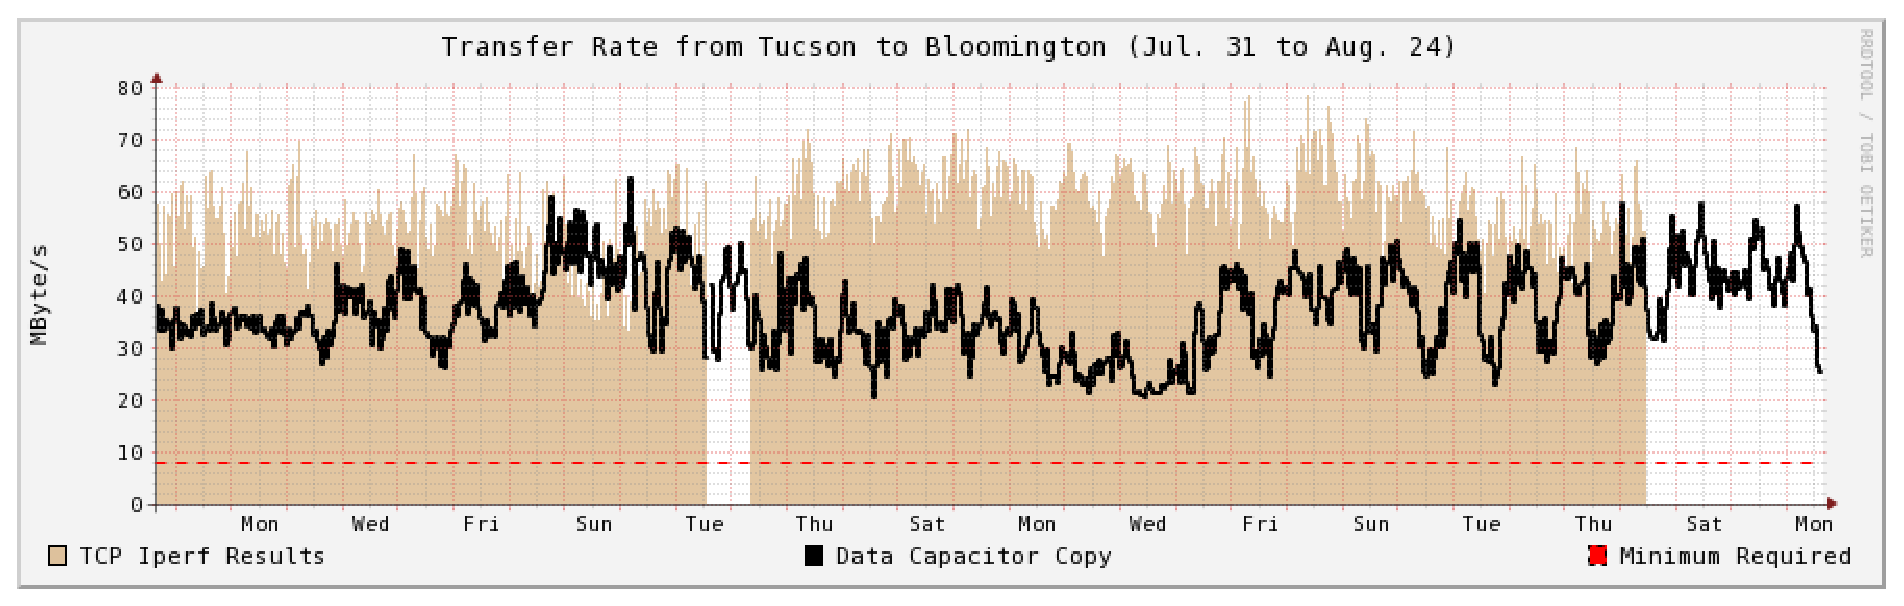
\includegraphics[width=6in]{network_throughput.eps}
\caption{Simulation Results}
\label{fig:network}
\end{figure*}

In our design the network is utilized for three main purposes; transferring data from the instrument to the Data Capacitor and archive, transmitting raw data and results during the processing phase, and distributing the data products to individual researchers. Since researches from all over the world can make use of the data products in the archive, it is difficult to characterize the network used to deliver the final data products, we will assume that typical requesters for data products will have less bandwidth than we can provide. Due to the fact that the network in this case is highly variable depending on the individual researcher's institution, we will focus on the first two of these purposes. 

The ODI instrument will be installed on the 3.5 meter telescope at the WIYN observatory on Kitt Peak. Once raw data is collected by the instrument it must be transferred to the facility that houses the short to mid-term storage and archive, in this case Indiana University. By using the Lustre filesystem over the WAN we allow the raw data to be transferred by a simple {\tt cp} command. Images can be copied over as they are taken or can be queued to balance the network load. If one assumes a data rate for the compressed raw data of 250 GB per night, then the nominal bandwidth required is 3 MB/s to transfer the data in a 24 hour period. We have performed tests transferring simulated data from the NOAO headquarters facility located in Tucson, Arizona near the Kitt Peak Observatory to the Data Capacitor at IU, and have found that the bandwidth from the NOAO headquarters is more than sufficient to transfer the raw data to the Data Capacitor. Figure \ref{fig:network} shows the results of these tests. The brown bars show the available bandwidth on the network, measured using the TCP iperf network testing software; the black line shows the data rate that can be achieved using standard copy operations with the Lustre file system of the Data Capacitor; the dashed red line represents the required
minimum network bandwidth to be able to transfer an average night's worth of ODI data to
the Data Capacitor in about 10 hours.

Using the iperf test tool, we determined that the available free bandwidth between Tucson
and Bloomington is between 30 and 80MB/s. With the Lustre file system of the Data Capacitor,
we can achieve a throughput between 20 and 60 MB/s over this connection. We measured
the throughput by copying an actual compressed image with a file size of roughly 1GB from NOAO to
the Data Capacitor. We copied one image every three minutes, for the entire test period throughout the month of August 2009.

For the distribution of raw data sets to the TeraGrid sites that will be used as compute facilities, we plan to use the TeraGrid network, a dedicated 10G research network. The same network will be used to return the data products resulting from the processing. The Data Capacitor has been used in conjunction with the TeraGrid network to facilitate distributed workflows at several TeraGrid sites including the Pittsburgh Supercomputing Center, the National Center for Supercomputing Applications \cite{henschel2010}, and the Texas Advanced Computing Center \cite{horowitz2010}; and will be used in a similar manner for ODI data. The amount of data to be transferred is of the same order as the amount of raw data, but will include the returned data products and calibration images so may exceed the raw data rate by a factor of two or more. However, this is not anticipated to be a problem with the TeraGrid network since it has an order of magnitude more bandwidth than the NOAO to IU network.

\subsubsection{Compute Facilities}

We will use supercomputers at several TeraGrid sites to provide the compute facilities to reduce the raw data and analyze the Tier 1 data. The TeraGrid is a national open scientific discovery infrastructure combining resources at eleven sites to create an integrated, persistent computational resource. Using high-performance network connections, TeraGrid provides integrated access to high-performance compute resources, and data resources and software tools around the country. Currently, TeraGrid resources include more than 2 petaflops of computing capability and more than 50 petabytes of online and archival data storage, with rapid access and retrieval over high-performance networks. With this combination of resources, the TeraGrid is the world's largest, most comprehensive distributed cyberinfrastructure for open scientific research \cite{teragrid}. In addition to Tier 1 automatic reductions TeraGrid compute resources will be used for user directed Tier 2 and Tier 3 reductions.

\subsubsection{Storage Systems}

We plan on using up to 200 TB of storage on the Data Capacitor, a system which provides researchers with a 535 TB file system to temporarily store and manipulate large data sets. The Data Capacitor consists of Dell 2950s running the Lustre file system, a detailed description of the deployment can be found in \cite{simms2007}. The Data Capacitor was used in a Bandwidth Challenge demonstration at SC07; this project was awarded first place with performance nearly twice the peak rate of the nearest competitor.

In our design the Data Capacitor will be used as the central storage facility for all storage needs during file transfer and processing. File transfers using the DC include transferring files from KPNO to the IU data center, interfacing with the IU MDSS archive and interfacing with the download servers. By mounting the Data Capacitor Lustre file system on a server at KPNO, we will be using the Data Capacitor to transfer files from KPNO to the IU Data Center. Section \ref{sec:network} outlines preliminary tests that show the feasibility. The Data Capacitor will serve as a back-end to the science gateway, providing the science gateway with fast access to image files and metadata. The Data Capacitor will also be used to make files available to TeraGrid compute facilities by directly mounting the Lustre file system. This will reduce the time for transferring files from the IU data center to the machines on the TeraGrid and speed up Tier 1 and Tier 2 data processing.

We plan to archive an average of 150 TB of data every year of the project, storing a total of 1.5 PB after 10 years of operation. The archive for ODI will be integrated into the IU Massive Data Storage Service (MDSS). MDSS utilizes High Performance Storage System (HPSS) software to manage a total capacity greater than 6.5 PB. HPSS, A hierarchical storage-management system by design, uses a hierarchy of storage media to provide massive, near-line data storage capacity. Data is written to a fast, front-end disk cache and migrated over time to robotic tape silos. IU was the first HPSS installation to implement distributed data movers, and now has redundant, distributed tape storage in Bloomington and Indianapolis connected via the I-Light network. Data written to IU's HPSS system is copied simultaneously to both locations, providing highly reliable disaster protection. 

\subsubsection{Pipeline Engine}

The pipeline engine is the part of the system containing the actual astronomical algorithms which will manipulate pixel values, calculate image statistics, and perform various transformations. We plan to utilize a heavily modified version of IRAF that will be updated to integrate seamlessly with the OGCE toolkit. IRAF, a software toolkit developed and maintained by NOAO, contains a vast number of algorithms that can carry out a number of astronomical analyses. It also has a number of graphical facilities that allow one to display and interactively manipulate images, however most of these graphical utilities will not function well over large network latencies and will need to be rewritten or heavily modified to work in the science gateway. 

\subsubsection{Pipeline Orchestration}

The algorithms of the pipeline engine will be orchestrated by the Open Grid Computing Environments (OGCE) toolkit. The OGCE toolkit is composed of several different pieces, called portlets, and will be coupled with the metadata catalog to track data processing and provenance. This catalog, the XML Metadata Concept Catalog (XMC Cat)\cite{jensen2008}, stores information about the contents of data files and workflows using a hybrid method developed at IU. In this method, the smallest pieces of information are stored in a relational database as name-value pairs, to support complex queries, but chunks of XML (collections of related data) are also stored. This is more flexible than storing the complete set of metadata in one XML document. The MyWorkspace Portlet provides an interface for users to the XMC Cat catalog. It creates a tree-based view for browsing workspace contents and also allows users to search and display the metadata associated with their workflows and data. The search interface is built dynamically, based on the hierarchy of the catalog. 

The Experiment Builder portlet uses a workflow composer application to allow the user to build workflows graphically. Input files, output files, and processing applications can be dragged into the work window and wired together to form a workflow that can then be launched on the TeraGrid. OGCE internals orchestrate the execution of the workflow. The same portlet can be used in monitoring mode to track the progress of a run. In order to include IRAF algorithms in the workflow composer, they must have a standardized interface to OGCE. To insure this we will wrap the algorithms with the Generic Factory Service (GFac).
 
GFac is a component that creates web services out of command-line science applications. Although portlets use web services to do the behind-the-scenes computations, existing science codes need not be converted to web services. Instead, they can be wrapped by a service that handles the communication between the portal and the science code, and does other useful work as well. These application services are created on an as needed basis, and are short-lived. This keeps the resources required to host and support multiple applications to a minimum.

The Grid Information, Proxy Management, Storage Resource Broker, and GRAM Job Submission Portlets take care of all the tasks needed to run jobs on the TeraGrid. These will obviously be used in the ODI gateway. In addition to these components, OGCE has portlets, applications, and tools to take care of tasks like administration of the gateway (e.g., adding new portlets), allowing users to modify their personal information and personalize the gateway. 

\subsubsection{Science Gateway}

The part of the system most visible to the astronomical community will be the science gateway. Science gateways provide a way for entire communities of users to access shared resources through a customized web-accessible interface. Since a science gateway is much more complex than an average website, it does more than simply provide information and links to other websites. Science gateways typically provide access to user data and data collections, community software, workflows, job execution, visualization, and social networking. They are especially useful in increasing productivity by shielding end users from the complexities of accessing data and running jobs on high-end compute resources with varying access mechanism.

Many scientific communities, in all fields, are beginning to use gateways to pool their resources and centralize expertise.  A list of science gateways that use the TeraGrid for compute power can be found at http://teragrid.org/gateways/. Of these, three are for astronomy: the Dark Energy Survey Data Management (DESDM) Gateway, the gateway for the Massive Pulsar Surveys using the Arecibo L-band Feed Array (ALFA), and the Asteroseismic Modeling Portal (AMP).  

The ODI gateway will be very similar in many ways to the LEAD Science Gateway (Linked Environments for Atmospheric Discovery), a TeraGrid Science Gateway developed at IU. LEAD is used by students and researchers for meteorological analysis and modeling. It was developed over 6 years as a research project. By building on this past work, co-opting, customizing, and modifying basic LEAD components, and adding our own specialized modules, we can build a unique and highly productive gateway optimized for ODI.

The ODI Science Gateway Prototype aligns quite nicely with the LEAD Gateway functionality and LEAD tools available through OGCE serve as natural building blocks for the ODI gateway. The tools include a data subsystem for cataloging raw images and investigation results, a workflow orchestration system, and all necessary dependencies. Back-end computation support on TeraGrid, fault tolerance, and workflow scheduling and execution are all built into the infrastructure. Since we will not have to construct this functionality from scratch, we can count the huge effort that has gone into developing these components as progress made prior to the project start date. Some of the major reusable components are described below.

\subsection{A Detailed Workflow for ODI Images}\label{sec:workflow}

Here we detail the steps in a workflow for processing a set of images. We follow the workflow from the acquisition of data at the telescope through Tier 2 processing directed by the end user. Each of the Tiers represent different levels of the reduction workflow and require different levels of cyberinfrastructure to support, see section \ref{sec:tiers} for a definition of each of the Tiers.

At IU, data will reside on both the Data Capacitor (DC) and the Massive Data Storage System (MDSS).
The Data Capacitor will host 200TB of short to mid-term storage for the analysis and production of Tier 1 and Tier 2 data products. Users will be granted quotas based on the projected amount of data that will be collected during their observations. In addition to quotas being granted to users with observing time, some amount of space will be made available to users interested in using archival data only. To prevent overruns on the Data Capacitor space, files that have been pulled from the archive and remain unused for some time will be deleted. However, the user will be able to quickly and easily restore them if they are needed again.

The MDSS will host the ODI archive, which will store all raw science images and calibration data.
Access to data in the archive will be restricted to the PI, and any users that he or she specifies, during the 18 month proprietary period following the observation. After this time, the raw data will become public. The PMD will contain searchable metadata entries for the data products, as well as the metadata for the processing itself (the workflow). The latter will allow the reproduction of data products from the raw archived data. 

Data transfer from the WIYN telescope to IU begins once an observation has been taken, the data and metadata files are available, and the transfer to the Data Capacitor has been queued. 
The summit facility will have a small disk buffer that will provide two weeks of raw data storage to smooth the data flow and mitigate interruptions due to network outages and system maintenance. As detailed in section \ref{sec:components} we have established a stable Data Capacitor mount from Tucson to IU which can meet the required data transfer rate. Next, the metadata file is ingested into the PMD. This is followed by copying the files from the Data Capacitor to the archive. Once this transfer is completed, the PMD communicates to the summit local buffer that the files have been replicated. They are then deleted from the local buffer and the transfer is removed from the queue.

New images are queued for Tier 1 processing by OGCE following the ingestion of the metadata and the verification of the files on the DC and MDSS. 
Based on the metadata associated with the image (e.g., observing mode, filter, moon phase, etc.), appropriate master calibrations and processing parameters are selected. The proper parameters for the processing engine and the TeraGrid resource best suited for the job are determined based on these selections. The workflow system then takes the input data, calibration data, and run parameters and generates the appropriate batch submission script for the TeraGrid resource that will run the job. For TeraGrid resources with Data Capacitor access the input data will already be available on the supercomputer. The job is executed on the TeraGrid resource and the results are written back to the Data Capacitor. The metadata is then updated with information about the job, as well as statistics of the result data. Once the Tier 1 processing has been confirmed the PI is notified. The PI can then log into the science gateway to view his or her Tier 1 processed data and begin Tier 2 processing or initiate a download.

Tier 1 data products will exist temporarily on the Data Capacitor, as it is a users' workspace. If the data are not accessed by the PI for some period of time, they will be migrated off of the DC. The processing metadata for the confirmed Tier 1 run will be saved so that the Tier 1 data products can be re-created using the same workflow, i.e., the same processing steps, parameters, and calibration data. This re-creation will occur seamlessly as needed, without the need for user interaction. The only indication of the reprocessing would be a delay in the initiation of a Tier 2 workflow or Tier 1 download.

Tier 1 data products will be made available to the PI and the public via the science gateway. One important and basic function of the gateway will be to enable users to browse and search their data.  When users log in to the gateway, they will be able to to see and select among their files by clicking in an expandable directory tree. Actually, the ''files'' will be complete images, the complex directory structure on the DC will be hidden from the end user, and the gateway will deal with all the details of matching files to images and displaying the proper metadata and thumbnails. When one clicks on a file in the tree, the metadata about that image (or table or other item) will be displayed. Thumbnails and larger versions of images will be available for display, as well.  
Searching for data will involve searching the metadata in the database to find observations, calibrations, or tables that have desired characteristics. One might, for example, search for all observations of M31 taken with a certain filter using a specific observing mode.

The ODI Science Gateway will also enable Tier 2 processing that is initiated and controlled by astronomers. To begin, the user will select one or more Tier 1 (or previously made Tier 2) images as input, then invoke the graphical workflow builder. From an astronomers point of view the workflow builder is probably the most novel aspect of the gateway, in that it allows a researcher to organize and process their data completely remotely by using an intuitive graphical interface.

Workflows consist of an operation or set of operations to be carried out on input data. Pre-made ODI workflows will be provided including stacking, differencing, slicing, object identification, photometry, and astrometry. Each will have a set of default parameters determined by an image processing expert to produce the best results for the broadest range of astronomical applications, but the user will be able to modify the settings if the need arises. A user will be able to select one or more pre-made workflows and arrange them in a desired order, connecting the input files to the the first task and wiring the others together, outputs to inputs (e.g., stack several narrow-band images and several broad-band images, then do a difference of the stacks). The arrangements can become quite complex. Forms in which to enter or edit required parameter settings will be constructed automatically. One will be able to save these user-made workflows for reuse and sharing.  Users will also be able to access the individual processing engine modules that make up the pre-made workflows, to compose more intricate workflows. In this way, users may exclude parts of a pre-made workflow that adversely influence their results.

Once a user has finalized his or her workflow and set all of the processing parameters, OGCE will dispatch the job to an appropriate TeraGrid resource. Although ODI image processing will occur on TeraGrid supercomputers, gateway users will not need TeraGrid accounts and will not have to deal with the (sometimes) complex process of running jobs on the TeraGrid. The gateway will submit jobs using a community account, take care of all the authorization and file movement details, and track resource usage by individuals. The workflow builder will also be able to monitor the progress of a running job. In ``monitoring mode,'' it will display notifications from the applications running on the TeraGrid. The status of all of a user's submitted jobs will also be displayed in the science gateway at login, and the user may elect to be notified by email when a job completes. 
 
Results from Tier 2 workflows will be stored in the user's workspace on the DC, available for download or for use as inputs to subsequent workflows. Before downloading, it will be possible to downsample or cut out sections of an image to limit the volume of data that has to be transferred then stored locally. Like Tier 1 data products, Tier 2 results will be moved off of the Data Capacitor after a period of time to allow the widest possible use of the system and to meet storage quotas. However, data products that are in use will not be deleted. Those that are deleted will still appear in the user's view in the science gateway but will be flagged as not needing to be recreated. Using the metadata saved for each workflow, data products will be reproduced as needed.

Although the proposed solution is similar in some ways to existing pipeline and archive facilities, our design incorporates several advances which make it a state-of-the-art solution. Early in the design process it was recognized that ODI data sets will be extremely large, complex, and difficult to work with, perhaps overwhelmingly so for individual users. Not only are the data volumes immense, but the complexity of dealing with 4096 {\tt .fits} extensions is significantly greater than what is experienced with typical mosaic imagers. It was also realized that simply delivering Tier 1 data products, via download or media as is done by many modern day pipeline systems, would not alleviate most of these difficulties. Due to these facts, we determined that the proposed solution should enable the end user to get as close as possible to the final scientific results of their workflow before requiring them to be responsible for receiving, storing and manipulating the data on their own. 

In this way the proposed solution differs substantially from most currently existing pipeline and archive facilities. Typically such facilities provide a data product, available for download or delivery, which a scientist can then manipulate to achieve his science goals. These facilities provide data products, {\bf not} a data reduction service, which is what this solution endeavors to do. In this respect, the solution will go far beyond current offerings. We will provide the data products, network connectivity, hardware, archival storage, and the necessary software toolkit to achieve many science goals. For many science programs the proposed system will truly be an end-to-end system.

Our design will also incorporate and enable additional features such as the inclusion of user contributed modules and community tools to enable and encourage collaboration on ODI projects. We will detail a process whereby users can develop their own modules that adhere to programming guidelines. After review by the pipeline scientists and programmers, these modules will be included and maintained by the pipeline staff. Community tools such as live messaging, forums, standardized workflows, etc. will be available via the science gateway. Users may, of course, decide to remain anonymous and opt out of these community tools if they wish. 

\section{Future Directions}\label{sec:future}

There are many potential applications of this new paradigm. Clearly, such a dramatic shift in the way that image processing is done will require significant changes in the preconceptions of many astronomers. As ODI is one of the first instruments to use this new approach, the adoption of it in the wider astronomical community will depend heavily on its success. To insure success of the project, several design, development and testing tasks must be completed. The various software and hardware components must be more tightly integrated and tested for fault tolerance. In addition, preliminary testing of the entire end to end system must be undertaken by several groups of potential users, which will test the limitations of the system in different ways. Once the system is functioning, ongoing support will be required to address any evolution in the underlying software and requests for additional functionality. In addition, education and outreach on the potential applications of the system and its proper uses in the astronomical community will be key. 

\section{Conclusions}\label{sec:conclusions}

In this paper we have introduced a potential new paradigm for astronomical image processing. For many astronomical image processing applications this new paradigm can result in increased efficiency and scientific discovery. The ODI instrument provides an ideal test case for this new way of image processing and analysis. By implementing a system using several different TeraGrid resources, orchestrated by the OGCE software toolkit, researchers can receive most of the functionality they currently have with desktop applications, such as IRAF, in a centralized system. The obvious benefits of such a system are lowering the barrier to entry for using a cutting-edge instrument, and reducing the amount of personal resources required by individual researchers. Less obvious, but perhaps even more compelling, are the benefits of access to a centralized repository of consistently processed data and the ability to effectively collaborate with other users of the instrument via the social networks aspect of the science gateway. Hopefully, this new vision represents a step into the future of astronomical image processing. 

\section*{Acknowledgments}

The authors would like to thank {\bf THANKS HERE}

This material is based upon work supported by the National Science Foundation under Grants No. ACI-0338618l, OCI-0451237, OCI-0535258, OCI-0504075, and CNS-0521433. This work was supported in part by Shared University Research grants from IBM, Inc. to Indiana University. Any opinions, findings and conclusions or recommendations expressed in this material are those of the authors and do not necessarily reflect the views of the National Science Foundation. 

\bibliographystyle{IEEEtran}
\bibliography{general}


% that's all folks
\end{document}


